

\documentclass[10pt,a4paper]{article}
\usepackage[utf8]{inputenc}
\usepackage[english]{babel}
\usepackage{amsmath}
\usepackage{amsfonts}
\usepackage{amssymb}
\usepackage{graphicx}
\usepackage{caption}
\usepackage{float}
\usepackage{array}
\usepackage{booktabs}	% for horizontal lines
\usepackage{varwidth}% http://ctan.org/pkg/varwidth
\usepackage{csvsimple} % automatic table generation from csv files
\usepackage{comment}
\usepackage[style=draft, backend=biber]{biblatex}

% new command for another subsection
\newcommand{\subsubsubsection}[1]{\paragraph{#1}\mbox{}\\}
\setcounter{secnumdepth}{4}
\setcounter{tocdepth}{4}

\addbibresource{../bibliography.bib}

\title{Chapter 2 - Fundamentals DRAFT}
\author{Weber Jakob}

\begin{document}
\maketitle

\section{Linear Models} \label{SectionLinModel}
	
\subsection{Definition and Model Assumptions}  \label{SubsectionLinModelDefAndAssump}

Given the set of data points $\{x_{i1}, ..., x_{iq}; y_i \}$ for $i = 1, ..., n$ , we aim to model the relation between the set of inputs or predictor variables $\{x_1, ..., x_q\}$ and the output $y$ with a function $f(x_1, ..., x_q)$ and an additional noise term $\epsilon$. Thus we obtain the model formulation as

\begin{equation}
	y_i = f(x_{i1}, ..., x_{iq}) + \epsilon_i
\end{equation}.

The goal is now the estimation of the unknown function $f$. For this, several assumptions on the model structure are needed:

\begin{enumerate}
	\item \emph{The unknown function $f$ is a linear combination of the input variables}
	
	The function $f(x_1, ..., x_q)$ is modeled as a linear combination of inputs, i.e.,
	\begin{align} \label{linCombOfInputs}
		f(x_1, ..., x_q) = \beta_0 + \beta_1 x_1 + ... + \beta_q x_q,
	\end{align}
	with unknown parameters $\beta_0, ..., \beta_q$, which need to be estimated. The model is therefore linear in its parameters as well as in its inputs. \cite{bishop2006patternRecognition} The parameter $\beta_0$ is called intercept or bias in the machine learning community. For centered data, i.e. $\mathbb{E}(x_i) = 0$, the intercept is equal to zero and can be neglected.
	
	Commonly, the linear model is represented in vector notation given by
	
	$$ y_i = f(x_{i1}, ..., x_{iq})  = x_i' \beta + \epsilon_i $$
	
	where $x' = (1, x_{i1}, \dots, x_{iq})$ and $\beta = (\beta_0, \dots, \beta_q)'$.
	
	\item \emph{Additive errors}
	
	The assumptions of additive errors leads to the following model structure
	\begin{align} \label{eq_linModelOneDim}
		y = x'\beta + \epsilon
	\end{align}
	This assumptions comes out to be quite restrictive, although it is reasonable for many practical applications.
\end{enumerate}

To estimate the unknown parameters $\beta$, we define the vectors $y = (y_1, ..., y_n)'$ and $\epsilon = (\epsilon_1, ..., \epsilon_n)'$ as well as the design matrix X, 

\begin{align}
	X = \begin{pmatrix}   1     & x_{11} & \dots & x_{1q} \\ 
					 	 \vdots &        &       & \vdots \\ 
				  		  1     & x_{n1} & \dots & x_{nq}  
		\end{pmatrix} \in \mathbb{R}^{n \times q+1}		
\end{align}

and generate $n$ equations like Eq.\ref{eq_linModelOneDim} which can be combined as 

\begin{align}
	y = X\beta + \epsilon.
\end{align}
We assume that the design matrix $X$ has full column rank, i.e. $rk(X) = q + 1 = p$, implying linear independence of the columns of $X$, which is necessary to obtain a unique estimator for the regression coefficients $\beta$. \cite{fahrmeir2013regression}

Another necessary requirement is that the number of data points $n$ is larger or equal to the number of regression coefficients $p$, which is equal to the statement that the linear system $y = X\beta$ is not under-determined.

In addition to the assumptions on the unknown function $f$, the necessary assumptions on the error term $\epsilon_i$ are the following:

\begin{enumerate}
	\item \emph{Expectation of the error} \\
	The errors have a mean of zero, i.e. $\mathbb E[\epsilon_i] = 0$

	\item \emph{Variances and correlation structure of the errors} \\
	We assume constant error variance with $\mathbb Var[\epsilon_i] = \sigma^2$ (homoscedasticity). Additionally, we assume that the errors are uncorrelated, which means $\mathbb Cov(\epsilon_i, \epsilon_j) = 0$ for $i \ne j$. These assumptions combined lead to the covariance matrix $\mathbb Cov(\epsilon) = \mathbb E(\epsilon \epsilon') 	= \sigma^2 I$.

	\item \emph{Gaussian errors} \\
	The errors follow at least approximately a normal distribution. With assumptions 1 and 2 we obtain that $\epsilon_i = \mathcal N(0, \sigma^2)$ 
\end{enumerate}

It follows from the model assumptions that 

\begin{equation}
\mathbb E[y_i] = \mathbb E [x_i'\beta + \epsilon_i] = x_i'\beta \\
\end{equation}
\begin{equation}
\mathbb V[y_i] = \mathbb V[x_i'\beta + \epsilon_i] = \mathbb{E}\big[(x_i'\beta + \epsilon_i - \mathbb{E}[y_i])^2\big] = \mathbb V[\epsilon_i] = \sigma^2 \\
\end{equation}
\begin{equation}
\mathbb Cov(y_i, y_j) = \mathbb Cov(\epsilon_i, \epsilon_j) = 0, 
\end{equation}
	
for the mean and variance of $y_i$, and the covariance between $y_i$ and $y_j$. With the additionally assumed Gaussian errors, we have

\begin{equation} \label{linModelAsDistribution}
y \sim \mathcal N(X\beta, \sigma^2 I).
\end{equation}

A linear model can therefore be interpreted as a normal distribution $\mathcal N(\mu, \sigma^2)$ with its mean given by $\mu = X\beta$ and its variance given by $\sigma^2 = \sigma^2 I$. To specify the linear model given through Eq.\ref{linModelAsDistribution}, we need to estimate the regression coefficients $\beta$ and the variance $\sigma^2$.


\subsection{Parameter Estimation}

The linear model given in Eq. \ref{linModelAsDistribution} has the unknown parameters $\beta$ and $\sigma$ which need to be estimated using given data. In the following part, the estimators $\hat \beta$ and $\hat \sigma$ are introduced, and their statistical properties are derived. 

\subsubsection{Estimation of the Regression Coefficients $\beta$}

The two main methods for the estimation of the regression coefficients in the context of linear models are

\begin{itemize}
	\item Method of Least Squares
	\item Method of Maximum Likelihood
\end{itemize}	

For Gaussian errors, the maximum likelihood estimator for the regression coefficients coincides with the least squares estimator. 

\subsubsubsection{The Method of Least Squares}

The unknown regression coefficients $\beta$ are estimated by minimizing the sum of squared error

\begin{equation} \label{MethodOfLS} 
\begin{split} 
\text{LS}(\beta) &=  \sum_{i=1}^n(y_i - x_i'\beta)^2 \\ 
	&= \sum_{i=1}^n\epsilon_i^2  \\
	&= \epsilon'\epsilon
\end{split}
\end{equation}

with respect to $\beta \in \mathbb{R}^p$. Rewriting of Eq.\ref{MethodOfLS} leads to the least squares criterion

\begin{equation*}
\begin{split}
\text{LS}(\beta) &= \epsilon'\epsilon \\ 
				 &= (y - X\beta)'(y - X\beta) \\ 
				 &= y'y - 2y'X\beta + \beta'X'X\beta.
\end{split}
\end{equation*}

The least squares criterion is minimized by setting its first derivative equal to zero and by showing that the matrix of second derivatives is positive definite. Applying the rules of differentiation we obtain

\begin{equation*}
\frac{\partial LS(\beta)}{\partial \beta} = -2X' y + 2X'X\beta.
\end{equation*}

The second derivative is given by

\begin{equation*}
\frac{\partial^2LS(\beta)}{\partial\beta \partial \beta'} = 2X'X
\end{equation*}
	
Since $X \in \mathbb{R}^{n \times p}$ for $p = q + 1$ has full rank (per assumption), the matrix $X'X$ is positive definite. The least squares estimate $\hat \beta_{LS}$ is then obtained by solving the so-called \emph{normal equations}

\begin{equation} \label{NormalEquations}
X'X \hat \beta = X'y.
\end{equation}


Since $X'X$ is positive definite and invertible, the normal equations in Eq.\ref{NormalEquations} have a unique solution given by the least squares estimate

\begin{equation} \label{LS_estimator}
\hat \beta_{LS} = (X'X)^{-1}X'y.
\end{equation}

\subsubsubsection{Maximum Likelihood Estimation}

Assuming normally distributed errors, i.e. $\epsilon \sim \mathcal N(0, \sigma^2I)$, the maximum likelihood estimators for the unknown parameters $\beta$ and $\sigma^2$ can be computed. Under the normality assumption the likelihood is defined as

$$L(\beta, \sigma^2) = \frac{1}{(2\pi\sigma^2)^{n/2}} \exp \Big( -\frac{1}{2\sigma^2}(y - X\beta)'(y - X\beta) \Big).$$

The log-likelihood is then given by

$$l(\beta, \sigma^2) = -\frac{n}{2}\log(2\pi) - \frac{n}{2}\log(\sigma^2) - \frac{1}{2\sigma^2}(y - X\beta)'(y - X\beta).$$

Thus, maximizing the log-likelihood with respect to $\beta$ is equivalent to minimizing the least squares criterion given in Eq.\ref{MethodOfLS}. The maximum likelihood estimator of $\beta$ is therefore equivalent to the least squares estimator in Eq.\ref{LS_estimator}.

\subsubsubsection{The Hat Matrix}

Using the least squares estimator $\hat \beta_{LS} = (X'X)^{-1}X'y$, we can estimate the mean of $y$ by 

$$\widehat{\mathbb{E}[y]} = \hat y = X\hat\beta_{LS}$$. 

This results in 

\begin{equation} \label{HatMatrix}
	\hat y = X(X'X)^{-1}X'y = Hy,
\end{equation}

with the matrix $H \in \mathbb{R}^{n \times n}$, which is called \emph{hat matrix}. Using the hat matrix, we can express the residuals $\hat \epsilon_i = y_i - \hat y_i$ in matrix notation as

$$\hat \epsilon = y - \hat y = (I - H) y.$$

The hat matrix $H$ has the following useful properties:

\begin{itemize}
\item  $H$ is symmetric.
\item $H$ is idempotent ( $H^2 = HH = H$ )
\item The rank of $H$ is equal to its trace.
\item $\frac{1}{n} \le h_{ii} \le \frac{1}{r}$, where $r$ represents the number of rows in $X$ with different $x_i$. If all rows are different, then $r = 1$.
\item The matrix $(I - H)$ is also idempotent and symmetric, with $rk(I - H) = n-p$.
\end{itemize}

The hat matrix is used in model selection techniques like cross-validation as well as in outlier detection and in the diagnostic plots for linear models.

\subsubsection{Estimation of the Variance $\sigma^2$}

The estimation of the variance $\sigma^2$ is necessary for the construction of confidence intervals of the regression coefficients and for the construction of prediction intervals. It is further used in all kinds of statistical tests. 

\subsubsubsection{Maximum Likelihood Estimation}

The variance $\sigma^2$ can be estimated using the maximum likelihood method by differentiation of the log-likelihood $l(\beta, \sigma^2)$ with respect to $\sigma^2$. The derivative is given by

$$\frac{\partial l(\beta, \sigma^2)}{\partial \sigma^2} = -\frac{n}{2\sigma^2} + \frac{1}{2\sigma^4}(y - X\beta)'(y - X\beta).  $$

Substituting the maximum likelihood estimator $\hat \beta$ for $\beta$ results in the maximum likelihood estimator for the variance $\sigma^2$ given by

\begin{equation} \label{sigma_ML}
	\hat \sigma_{ML}^2 = \frac{(y-X\hat\beta)'(y - X\hat\beta)}{n} = \frac{\hat\epsilon' \hat\epsilon}{n}.
\end{equation}

This estimator for $\sigma^2$ is rarely used since it is biased, i.e. $\mathbb{E}[\sigma^2_{ML}] \ne \sigma^2$. 

\subsubsubsection{Restricted Maximum Likelihood Estimation}

Using $\mathbb{E}(\hat\epsilon' \hat\epsilon) = (n - p)\sigma^2$, we obtain for the restricted maximum likelihood estimation of the variance $\sigma^2$ the following:

\begin{equation} \label{sigma_REML}
	\hat \sigma^2_{REML} = \frac{1}{n-p} \hat\epsilon' \hat\epsilon,
\end{equation}

which is the commonly used estimator for $\sigma^2$. The restricted maximum likelihood estimator for the variance is in general less biased. Therefore, it is a better choice to use this estimator.

\subsection{Model Selection Techniques, Model Choice Criteria and Regularization}

Linear models can be used to generate models using a large number of input or predictor variables. The challenge is then to decide which of these variables to include in the model. 

On way of comparing various models, i.e models using different sets of variables, is the use of model choice criteria, e.g. Mallow's CP or AIC. Generally, these criteria can be split in two parts. The first part measures the goodness of fit, e.g. using the sum of squared errors, while the second part measures the complexity of the model. 

Most model choice criteria are based on the sum of squared prediction error $SPSE$. Therefore, the derivation of the sum of squared prediction error $SPSE$ is given first.

We assume given data $\{ x_{i1}, \dots, x_{iq}; y_i\}$ for $i =1, \dots, n$. Further, we assume that the expectation $\mathbb{E}[y_i] = \mu_i$ and the variance $\mathbb{V}ar[y_i] = \sigma^2$. Using the $q$ variables $x_i$ we can generate the corresponding design matrix $X$ for the linear model $y = X\beta$. The least squares estimator for $\beta$ is then given by

$$\hat \beta_{LS} = (X'X)^{-1}X'y.$$

The data $y$ can be interpreted as random variable. We can then define an estimator $\hat  y$ for the vector $\mu$ of expectations $\mu_i = \mathbb{E}[y_i]$ by

$$\hat  y = X \hat \beta.$$

The following properties the $\hat y$ hold:

\begin{itemize}
	\item $\mathbb{E} [\hat y] = X(X'X)^{-1}X'\mathbb{E}[y]$
	\item $\mathbb Cov(\hat y) = \sigma^2 X(X'X)^{-1}X'$
	\item $\sum_{i=1}^n \text{Var} [\hat y_i] = \sigma^2 \text{tr}(X(X'X)^{-1}X') = \vert M \vert \sigma^2$, where $M$ represents the number  of used variables.
	\item Sum of Mean Squared Error
		\begin{equation}  
		\begin{split} 
		\text{SMSE} &= \sum_{i=1}^n \mathbb{E}[\hat y_i - \mu_i]^2 \\
				    &= \sum_{i=1}^n \mathbb{E}\big[(\hat y_i - \mathbb{E}[\hat y_i]) + (\mathbb{E}[\hat y_i] - \mu_i) \big]^2 \\
				    &= \vert M \vert\sigma^2 + \sum_{i=1}^n(\mathbb{E}[\hat y_i] - \mu_i)^2.
		\end{split}
		\end{equation}
\end{itemize}

If we now assume new data $\{ x_{i1}, \dots, x_{ik}; \ y_{n+i} = \mu_i + \epsilon_{n+i}\}$ for $i = 1, \dots, n$, we can use the estimator $\hat  y$ as a prediction for these new observations. We can therefore derive the sum of the expected squared prediction errors SPSE, given by

\begin{equation}
\begin{split}
	\text{SPSE} &= \sum_{i=1}^n \mathbb{E}[y_{n+i} - \hat y_i]^2 \\ 
				&= \sum_{i=1}^n \mathbb{E}\big[(y_{n+i} - \mu_i) - (\hat y_i - \mu_i)\big]^2 \\ 
				&= \sum_{i=1}^n \mathbb{E}[y_{n+1} - \mu_i]^2 + 2\mathbb{E}[(y_{n+1} - \mu_i)(\hat y_i - \mu_i)] + \mathbb{E}[hat y_i - \mu_i]^2 \\
				&= \sum_{i=1}^n\mathbb{E}[y_{n+i} - \mu_i] + \sum_{i=1}^n(\mathbb{E}[\hat y_i] - \mu_i)^2 \\ 
				&= n\sigma^2 + SMSE \\ 
				&= n\sigma^2 + \vert M \vert \sigma^2 + \sum_{i=1}^n(\mathbb{E}[\hat y_i] - \mu_i)^2.
\end{split}
\end{equation}


The sum of the expected squared prediction error can be split into three parts

\begin{itemize}
	\item \emph{Irreducible Prediction Error Term} \\
	This term cannot be reduced through model selection techniques since it only contains the number of data points $n$ and the variance $\sigma^2$.

	\item \emph{Variance Term} \\
	The second term contains the number of used variables $\vert M \vert$ as well as the variance $\sigma^2$. It can therefore be reduced by using a smaller number of variables.
	
	\item \emph{Squared Bias Term} \\
	The last term can be interpreted as bias. It can be reduced by increasing the model complexity.
\end{itemize}

The sum of expected squared prediction error is an example of the bias-variance trade-off, which is characteristic for all statistical models. It states that by increasing model complexity, the bias is reduced but instead the variance is increased. On the other side, by decreasing model complexity, the variance of the model is reduced, but the bias is increased. \cite{bishop2006patternRecognition}

%[https://en.wikipedia.org/wiki/Bias–variance_tradeoff](https://en.wikipedia.org/wiki/Bias%E2%80%93variance_tradeoff)

In practice, the true value for the SPSE is not accessible since $\mu_i$ and $\sigma^2$ are unknown. Therefore, we need to estimate the SPSE. This can be done by using one of the following two strategies:

\begin{enumerate}

	\item \emph{Estimate SPSE using new and independent data} \\	
	If new observations are available, the SPSE can be estimated by
	$$\widehat{\text{SPSE}} = \sum_{i=1}^n (y_{n+i} - \hat y_i)^2.$$
	These new observations can also be some held-out validation data from a train-validation split of the given data. 
	
	\item \emph{Estimate SPSE using existing data} \\
	When using existing data, the estimate for the SPSE is given by the squared error and an additional error term depending on the estimated variance and the model complexity. The estimate is thus given by
	$$\widehat{\text{SPSE}} = \sum_{i=1}^n(y_i - \hat y_i)^2 + \vert M \vert \hat \sigma^2.$$
\end{enumerate}

Typically used model choice criteria follow the basic idea of the SPSE.

\subsubsection{Model Choice Criteria}

\subsubsubsection{Corrected Coefficient of Determination $R^2_{corr}$}

The corrected coefficient of determination is an is an improvement over the coefficient of determination $R^2$, which is defined as 

$$R^2 = 1 - \frac{\sum_{i=1}^n \hat \epsilon_i^2}{\sum_{i=1}^n (y_i - \bar y)^2},$$

where $\bar y$ is defined as the mean value of $y$. The major drawback of $R^2$ is that it will never decrease when further predictors are included in the model, e.g. the $R^2$ of a model using $\{x_1, x_2, x_3\}$ is always larger or equal the $R^2$ of a model using $\{x_1, x_2\}$, even if the variable does not enhance the prediction quality. 

The corrected coefficient of determination $R_{corr}^2$ reduces this problem by an correction term depending on the  number of parameters and is given by

$$R_{corr}^2 = 1 - \frac{n-1}{n-p}(1-R^2). $$

The corrected coefficient of determination is a standard output parameter in many statistical programs and may be used to compare even models with different number of used variables. 

\subsubsubsection{Mallow's Cp}

Mallow's complexity parameter bases directly on the ideas specified for the estimation of the SPSE and is given by

$$\text C_p = \frac{\sum_{i=1}^n (y_i - \mathbb{E}[y_i])^2}{\hat \sigma^2} - n + 2 \vert M \vert,$$

where $M$ is again the number of used parameters. Lower values of Mallow's $\text C_p$ correspond to a better model fit.

\subsubsubsection{Akaike Information Criterion}

The AIC is among the most used model choice criteria and defined by

$$\text{AIC} = -2 l(\hat \beta_{ML}, \hat \sigma^2_{ML}) + 2(\vert M \vert +1)$$

where $l(\hat \beta_{ML}, \hat \sigma^2_{ML})$ is the value of the log-likelihood at its maximum. We again have the standard model choice criteria structure of a data dependent term, here the maximal log-likelihood, and a model dependent term given. 

The log-likelihood for a linear model assuming Gaussian errors is given by

$$-2l(\hat\beta_{ML}, \hat \sigma_{ML}^2) = n \log(\hat \sigma_{ML}^2) + n.$$

Therefore, neglecting the constant value $n$, the AIC evaluates to

$$\text{AIC} = n \log(\hat \sigma^2_{ML}) + 2(\vert M \vert + 1).$$

Lower values of AIC correspond to a better model fit. 

\subsubsubsection{Bayesian Information Criteria}

The BIC is similar to the AIC, but it penalizes more complex models much harder than the AIC. In its general form, it is given as 

$$\text{BIC} = -2l(\hat\beta_{ML}, \hat \sigma^2_{ML}) + \log(n) (\vert M \vert + 1).$$

Again, assuming Gaussian errors for a linear model and neglecting the constant term $n$, the BIC evaluates to

$$\text{BIC} = n\log(\hat \sigma_{ML}^2) + \log(n)(\vert M\vert + 1).$$

Lower values of BIC correspond to a better model fit.

\subsubsubsection{Cross Validation}

The basic idea of cross validations is to split the existing data set into multiple smaller ones and to fit one model to each of these smaller data sets. These models are then evaluated by the calculation of the SPSE on the data which it was not trained on. The model which has the smallest error is then chosen as final estimate. 

A special case of cross validation is the "leave-one-out" cross validation, where all but one data point are used for training and the model is then evaluated on this held-out data point. This seems to be quite expensive, since one needs to estimate one model per data point. 

However, in the context of linear models, it can be shown that the cross validation score can be computed using one estimator trained on all data $y$ and the hat matrix $H = X(X'X)^{-1}X'$. The cross validation score is then given by

$$\text{CV} = \frac{1}{n} \sum_{i=1}^n\big( \frac{y_i - \hat y_i}{1 - h_{ii}}\big)^2.$$

where $h_{ii}$ denotes the diagonal elements of the hat matrix and $hat y_i$ is defined as the prediction for the input $x_i'$. A lower cross validation score corresponds to a better model fit. \cite{golub1979}

An approximation to the cross validation score is given by the so-called Generalized Cross Validation score. It is mainly used in the context of non-parametric regression or when the hat matrix $H$ is numerically expensive to compute. In the GCV score, the diagonal elements of the hat matrix $h_{ii}$ are replaced by the mean of the trace of $H$. The GCV score is then given by

$$\text{GCV} = \frac{1}{n}\sum_{i=1}^n \Big( \frac{y_i - \hat y_i}{1 - \text{trace(H)}/n}\Big)^2.$$

The numerical advantage comes from the fact that the trace of a product of matrices is not changed when cyclically permuting the product of matrices, i.e. $\text{trace}(H) = \text{trace}(X(X'X)^{-1}X') = \text{trace}(X'X(X'X)^{-1})$. The trace can therefore be computed from the product of two matrices of shape $p\times p$. \cite{fahrmeir2013regression}

\subsubsection{Model Selection Techniques}

To make use of the various model choice criteria, some algorithmic approach to model selection needs to be given. The most commonly used are given below. We always start with a candidate model. \cite{fahrmeir2013regression}

\subsubsubsection{Forward Selection}

We start with a candidate model which includes a small number of variables. In each iteration of forward selection, an additional variable is included into the candidate model.  The added variable is the one with leads to the largest reduction of a predefined model choice criteria. The algorithm stops, if no further reduction is achieved.

\subsubsubsection{Backward selection}

We start with a candidate model which includes all variables. In each iteration of backward selection, we eliminate the variable from the model which provides the largest reduction of a predefined model choice criteria. The algorithm stops, if no further reduction is possible. 

\subsubsubsection{Step-wise Selection}

In step-wise selection, forward and backward selection are combined to enable the inclusion and deletion of a variable in every operation. The algorithm stops, if no further reduction is possible.

\subsubsection{Regularization}

Model selection can also be achieved using regularization techniques. In general, regularization restricts the parameter space by adding some penalty term depending on the complexity of the model. This leads to the penalized least squares criterion

$$\text{PLS}(\beta) = \lVert y - X\beta\rVert^2 + \lambda *\text{pen}(\beta)$$

where $\lambda$ is the so-called smoothing parameter and $\text{pen}(\beta)$ is the penalty term. The two most commonly used forms of regularization are the Ridge Regression and the Lasso Regression. Both are explained in detail in the following.

\subsubsubsection{Ridge Regression}

In Ridge regression, the penalty term in the penalized least squares criterion is given by the squared $L_2$-norm of the coefficient vector $\beta$. The objective function to minimize is therefore given by

$$\text{PLS}(\beta) = \lVert y - X\beta\rVert^2 + \lambda \beta'\beta$$

which the closed form solution 

$$\hat\beta_{PLS} = (X'X + \lambda I_p)^{-1}X'y,$$

where $I_p \in \mathbb R^{p \times p}$ is the identity matrix. The additional penalty term in Ridge regression leads to smaller parameter estimates $\hat \beta_{PLS}$ compared to the un-penalized estimate $\hat \beta_{LS}$. For large values of the smoothing parameter $\lambda$, the parameter estimates will be converge towards, but never reach, zero. 

Ridge regression is commonly used for design matrices $X$ that are close to nonlinear or when the input dimension is high. \cite{hoerl1970ridge}

\subsubsubsection{Lasso Regression}

One drawback of Ridge regression is that it does not produce sparse solutions, i.e. all estimated coefficients will be different from zero. Lasso regression tackles this problem by the use of the $L_1$-norm as penalty term. The penalized least squares objective function is then given by

$$\text{PLS}(\beta) = \lVert y - X\beta \rVert + \lambda*\sum_{i=1}^k\vert \beta_i\vert,$$

where $\lambda$ again plays the role of a smoothing parameter. No closed form solution is available for Lasso regression. The Lasso estimates  $\hat \beta_{Lasso}$ are calculated using either quadratic programming techniques, given in \cite{tibshirani1996lasso}, or least angle regression, given in \cite{efron2004leastangleregression}. Ridge regression penalized large coefficients much stronger than Lasso regression, while for small coefficient values, the Lasso penalty has much more influence. \cite{tibshirani1996lasso}


\section{Splines} \label{SectionSplines}
	
In it's most general definition a spline is a piece-wise polynomial defined on a sequence of knots. This definition is quite general. Therefore, there exist a large variety of splines, ranging from regression splines in \cite{eubank1990regressionsplines}, over B-splines in \cite{deBoor1978practicalGuideToSplines} to natural cubic splines and many more.

\subsection{B-Splines}

We lay the focus on the definition and use of B-splines, which are constructed from polynomial pieces in a recursive manner. The following figure shows a simple example of a B-spline of degree 1 on the left. It consists of two linear pieces, one from $x_1$ to $x_2$ and the other from $x_2$ to $x_3$. Everywhere else, the B-spline is equal to zero. This locality is a very attractive feature of B-splines. In the right part of the figure, a B-spline of degree 2 is shown, which consist of three quadratic pieces. At the joining points, the values as well as the first derivatives of the quadratic pieces are equal. 

\begin{figure}[H]
	\centering
	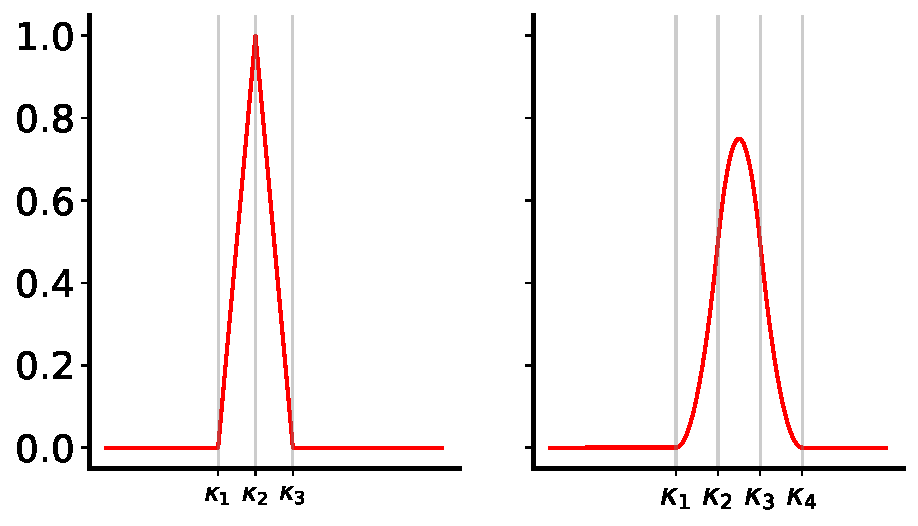
\includegraphics[width=\columnwidth]{../thesisplots/linear_and_quadratic_spline.pdf}
	\caption{Linear and Quadratic Spline}
	\label{fig:lin_and_quad_spline}
\end{figure}


The general properties of a B-spline of degree $m$ are the following:

\begin{itemize}
	\item It consists of $m+1$ polynomial pieces of degree $m$, e.g. a cubic spline ($m=3$) consists of 4 cubic pieces.
	\item The pieces join at $m$ inner knots.
	\item At these knots, the derivatives up to order $m-1$ are continuous.
	\item The B-spline is positive on the domain spanned by $m+2$ knots, everywhere else it is zero.
	\item At every given $x$, only $m+1$ B-splines are non-zero.
\end{itemize}

The collection of $k$ B-splines of degree $m$ over a sequence of $k+2(m-1)$ knots is called B-spline basis. The $2(m-1)$-knots are the boundary knots while the $k$ knots are the interior knots. The knots can either be an equidistant sequence, which facilitates the construction and estimation of the coefficients, or a non-equidistant sequence.

A smooth function can then be represented using the basis function approach given by

$$f(x) = \sum_{i=1}^k B_i^m(x) \beta_i $$

using the B-spline basis $B_i^m(x)$ which is defined recursively using the knot sequence $x_i = \{x_1, \dots, x_{k+2(m-1)}\}$ according to \cite{deBoor1978practicalGuideToSplines} as follows:

$$B_i^m(x) = \frac{x - x_i}{x_{i+m} - x_i} B_i^{m-1}(x) + \frac{x_{i+m+1} - x}{x_{i+m+1} - x_{i+1}} B_{i+1}^{m-1}(x)$$

and

$$B_i^0(x) = \begin{cases} 1, & x_i \le x < x_{i+1} \\ 0, & \text{otherwise} \end{cases}.$$

The use of B-splines as basis functions for uni-variate or non-parametric regression is very attractive. A linear combination of cubic B-splines gives a smooth curve (first and second order derivatives are continuous). A further advantage of B-splines is that once the basis is given, the coefficients can be estimated using the Least Squares algorithm. The least squares formulation for splines is the given by

$$Q(\beta) = \lVert y - X\beta\rVert^2$$

for the B-spline basis $X \in \mathbb{R}^{n \times k}$ for $n$ data points and $k$ splines, which leads to the estimated coefficients 

$$\beta_{LS} = (X^TX)^{-1}X^T y$$

Therefore, the estimation is computationally efficient and easy to implement since closed-form solutions exists. Further, the advanced theoretical framework of linear models can be applied to calculate e.g confidence intervals for the regression coefficients and the prediction.

B-splines of appropriate order  produce smooths curves, where the smoothness is determined by the number of splines used. For a low number, the curve will be quite smooth, but with a large data error. When using a high number of splines, the data error will be small but the variance of the curve will be large. This is an example of the bias-variance trade-off, a classical problem of regression and machine learning. It is therefore necessary to introduce some kind of regularization. \cite{deBoor1978practicalGuideToSplines}  

\subsection{P-Splines} \label{SubsectionPspline}

P-splines where introduced by Eilers and Marx in \cite{eilers1996flexible} to tackle the problem introduced above. Eilers and Marx simplified and generalized the idea of \cite{osullivan1986statistical}, who introduced a penalty on the integral of the squared second derivative of the estimated spline to penalized wiggly function estimates. Eilers and Marx proposed to use equidistant knots and to base the penalty on finite differences of order $d$ of the coefficients of adjacent B-splines. In \cite{osullivan1986statistical}, O'Sullivan implicitly used a modified second-order penalty. The finite differences of order $1$ for $k$ splines are given by

$$\Delta^1 \beta = \sum_{j=2}^{k-1} \beta_{j} - \beta_{j-1}$$

and in matrix form

$$\Delta^1 = D_1 = \begin{pmatrix} -1 & 1 \\ & \ddots & \ddots \\   \end{pmatrix} \in \mathbb{R}^{k-1 \times k}.$$

This leads to the penalized least squares formulation

$$Q(\beta; d) = \lVert y - X\beta\rVert^2 + \lambda_s \mathcal J_s(\beta;d)$$

where $\lVert y - X\beta \rVert^2$ is the mean squared error on the data for the spline smooth, $\mathcal J_s(\beta;d) = \beta^T D_d^T D_d \beta$ is the smoothness penalty term and $\lambda_s$ is the smoothness parameter effect of the smoothing penalty. The estimated coefficients are then given by

$$\beta_{LS,p} = (X^TX + \lambda_s D_d^T D_d)^{-1}X^Ty$$

The main advantage of P-splines is their easy set up. This advantage is diminished if uneven knot placement is chosen. 

\subsection{Tensor-Product Splines}

Tensor-product splines can be seen as the multi-dimensional extension of univariate splines. The basic approach is to start with a spline basis for each dimension and construct the tensor-product spline from these. 

We examine an example for two input dimensions $x_1$ and $x_2$. Assume that we have bases available for representing the functions $f_1(x_1)$ and $f_2(x_2)$ given by

$$f_1(x_1) = \sum_{i=1}^{k_1} \alpha_i a_i(x_1), \quad f_2(x_2) = \sum_{j=1}^{k_2} \beta_j b_j(x_2),$$

where $\alpha_i \in \mathbb{R}^{k_1}$ and $\beta_j \in \mathbb{R}^{k_2}$ are the coefficients and $a_i(x_1)$ and $b_j(x_2)$ are the known basis functions. To allow the function $f_1(x_1)$ to smoothly vary with $x_2$, its coefficients $\alpha_i$ must vary smoothly with $x_2$. By using the already available basis for representing smooth functions in $x_2$, we can write

$$\alpha_i(x_2) = \sum_{j=1}^{k_2} \beta_{ij} b_j(x_2)$$

which leads to

$$f_{1,2}(x_1, x_2) = \sum_{i=1}^{k_1} \sum_{j=1}^{k_2} \beta_{ij} b_j(x_2) a_i(x_1).$$

For any set of data $(x_{1i}, x_{2i})$ for $i = 1, \dots, n$ there is a relationship between the model matrix $X$ of the tensor-product smooth and the marginal model matrices $X_1$ and $X_2$, which is given by 

$$X_i = X_1 \otimes X_2.$$

where $\otimes$ indicates the use of the Kronecker product, $X_1$ denotes the B-spline basis for dimension $1$ and $X_2$ denotes the B-spline basis for dimension $2$. \cite{wood2006GAM} The model matrix for the tensor-product smooth is therefore given by the Kronecker product of the marginal model matrices. 

This approach can in theory be continued for as much input dimensions as required. In practice, modeling more than two input dimensions using tensor-product splines becomes infeasible because if the enormous increase in used basis functions. A smoothness penalty term for tensor-product splines can also be constructed using the Kronecker product. Further explanations are given in Chapter 3.


\section{Structured Additive Regression}

We have again some given data $\{x_{i1}, \dots, x_{iq}; y_i\}$ for $i = 1, \dots, n$, where we want to model the generally non-linear relationship between the input data $\{x_{i1}, \dots, x_{iq}\}$ and the output $y$ by some function $f(x_1, \dots, x_q)$.  Using, e.g. high-dimensional tensor-product splines, to model the function is computationally expensive, since the number of regression coefficients increases exponentially.

To circumvent this problem, we now assume the restrictive structure of additive models, given by

\begin{equation} \label{addRegBaseEquation}
	f(x_1, \dots, x_q) = f_1(x_1) + \dots + f_q(x_q). 
\end{equation}
Hence, we use one smooth function per input dimension and assume an additive structure. \cite{fahrmeir2013regression} Using the concepts introduced in Chapter \ref{SectionSplines}, we obtain for each smooth function a linear model

$$f_i(x_i) = X_i \beta_i$$

where $X_i \in \mathbb R^{n \times k_i}$ is the B-spline basis using $k_i$ splines for input dimension $i$ and $\beta_i \in \mathbb R^{k_i}$ are the coefficients to be estimated. We can also use the already described penalization approaches given in Chapter \ref{SubsectionPspline}. 

The model given in Eq. \ref{addRegBaseEquation} does not contain interaction terms between variables. Nevertheless, these can be easily introduced for 2 dimensions using tensor-product splines without an overflowing increase of the number of regression coefficients.

We can then write the structured additive model in matrix notation as 

\begin{equation} \label{structAddRegressionEquation}
	y = X_1\beta_1 + \dots + X_q\beta_q + \sum_{i=1}^{n_{interact}} X_{tps, i} \beta_{tps,i} + \epsilon
\end{equation}

using the error term $\epsilon$ and $n_{interact}$ as the number of interactions to include via tensor-product spline bases $X_{tps,i}$. This can be solved using ordinary least squares. If we choose to include penalization, we can solve this using penalized least squares. 

Using the notation in Eq. \ref{structAddRegressionEquation} the theoretical framework of linear models can be applied to structured additive regression models. Therefore, the assumptions given in Chapter \ref{SubsectionLinModelDefAndAssump} on the error term, as well as on the model functions are used. \cite{fahrmeir2004penalized}


\printbibliography
	
\end{document}